\documentclass{hbrs-ecta-report}

\usepackage{float}
\usepackage{placeins}
\begin{document}

\conferenceinfo{H-BRS}{2017}

\title{Neuroevolution: Simple Hill Climbing}
\subtitle{[Example Report]}

\numberofauthors{2}
\author{
\alignauthor
.
}

\date{today}
\maketitle
\begin{abstract}
Short summary: in \textbf{very few} sentences, describe what was asked, what you did and what the results were
\end{abstract}

%% ------------------------------ GENERAL NOTES ------------------------------ %%
\section{General Notes}

%% ------------------------------ REPORT STRUCTURE ------------------------------ %%
\FloatBarrier
\newpage
\subsection{Figure}

\begin{figure}[ht!]
\centering
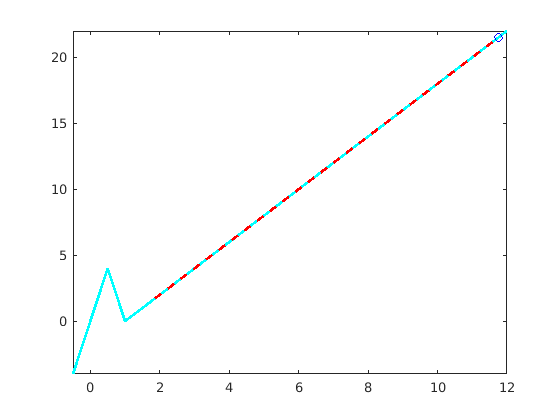
\includegraphics[width=\linewidth]{img/plot_fit_max.png}
\caption{Development of average mean square error, comparing NEAT and ESP}
\label{fig:1} 
\end{figure}

\FloatBarrier
\section{Conclusion}


\bibliographystyle{abbrv}
\bibliography{HeteroNEAT} 
\end{document}
}